%%
%% 2020 graphische Interpretation linearer Gleichungen (TALS nSpire)
%%


\newpage
\subsection{Graphische Interpretation}
Graphische Interpretation der Grundform:

In der Form
$$ax+b=0$$
ist $a$ die Steigung\footnote{Steigung: Eine Einheit nach rechts: Um wie viele Einheiten steigt die Gerade an?} der Geraden und $b$ der Abschnitt\index{Achsenabschnitt} auf der $y$-Achse\footnote{$y$-Achsenabschnitt: Wo schneidet die Gerade die $y$-Achse.}:

\bbwCenterGraphic{6cm}{allg/gleichungen/img/LineareGleichungsfunktion.png}
%  \begin{center}
%   \raisebox{-1cm}{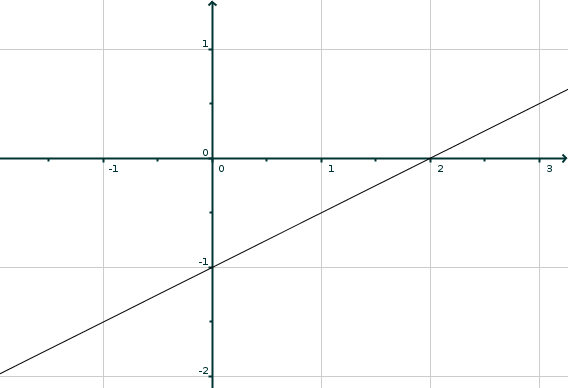
\includegraphics[width=6cm]{img/LineareGleichungsfunktion.png}}
%  \end{center}

  \paragraph{Charakteristische Punkte}
  Die charakteristischen Punkte (spezielle Punkte) der linearen
  Funktion in Grundform sind

  \begin{itemize}
  \item $b$ = $y$-Achsenabschnitt: Wo schneidet die Gerade die $y$-Achse?
  \item $a$ = Steigung der Geraden pro eine Einheit nach rechts (in $x$-Richtung)
  \item $\frac{-b}{a}$ = Lösung der Gleichung $ax+b=0$. Dies ist der $x$-Achsenabschnitt.
  \end{itemize}

